%=======================================================================
%  CSE558 Data Science - Midterm Project Report Template
%  Monsoon 2026, IIIT-Delhi
%
%  How to use this template
%   1. Set your project title in the EDIT THIS block below.
%   2. Replace everything in LIGHT BLUE with your own text and numbers.
%      The numbers in the example are made up for illustration.
%   3. Grey italic lines are instructions. Delete them as you write, or
%      hide them all at once with \showhintsfalse.
%   4. Upload your plots to the project and put their file names in
%      \figfile{...}{...}. Until a file exists, a labelled box is shown.
%
%  Sections 1-5 follow items 1-5 of the report guidelines; Section 6 is
%  the limitations of your analysis. The link to your code (item 6) goes
%  at the top. At most 8 pages.
%  Compile with pdfLaTeX (Overleaf's default setting works), twice.
%=======================================================================
\documentclass[10pt,a4paper,twocolumn]{article}

%========================= EDIT THIS =========================
% Your project title: it sets the heading AND the PDF's title.
\newcommand{\projecttitle}{Observed repayment outcomes in LendingClub accepted loans}
\newif\ifshowhints
\showhintsfalse      % \showhintsfalse hides every grey instruction line
%=============================================================

%-------------------------------------------- fonts (no need to edit)
\usepackage[T1]{fontenc}
\usepackage[scaled=0.92]{helvet}\renewcommand{\familydefault}{\sfdefault}
%----------------------------------------------------------- packages
\usepackage[margin=18mm,bottom=20mm,columnsep=7mm]{geometry}
\usepackage{amsmath}
\usepackage{xcolor}
\usepackage{graphicx}
\usepackage{tabularx}
\usepackage{array}
\usepackage{booktabs}
\usepackage{enumitem}
\usepackage{titlesec}
\usepackage{needspace}
\usepackage[font=small,labelfont=bf]{caption}
\usepackage[hidelinks]{hyperref}
\hypersetup{pdftitle={\projecttitle},
            pdfsubject={CSE558 Data Science, Monsoon 2026: Midterm Project Report}}

%------------------------------------------------------------- layout
\definecolor{eg}{HTML}{7396C4}         % worked example (light blue)
\definecolor{hintgrey}{gray}{0.58}     % instructions (light grey)

\titleformat{\section}{\normalfont\large\bfseries}{\thesection.}{0.5em}{}
\titlespacing*{\section}{0pt}{12pt}{3pt}
\titleformat{\subsection}{\normalfont\normalsize\bfseries}{\thesubsection}{0.5em}{}
\titlespacing*{\subsection}{0pt}{10pt}{2pt}
\newcommand{\sectionbreak}{\needspace{10\baselineskip}}
\newcommand{\subsectionbreak}{\needspace{10\baselineskip}}

\setlength{\parindent}{0pt}
\setlength{\parskip}{4pt}
\setlist{leftmargin=1.2em, itemsep=2pt, topsep=2pt, parsep=0pt}
\renewcommand{\arraystretch}{1.25}
\setlength{\tabcolsep}{4pt}
\newcolumntype{L}[1]{>{\raggedright\arraybackslash}p{#1}}
\newcolumntype{Y}{>{\raggedright\arraybackslash}X}
\newcolumntype{K}[1]{>{\raggedright\arraybackslash\bfseries\boldmath}p{#1}}  % bold labels

%--------------------------------------------------------- shorthands
% Instruction line. Delete these as you fill the template in.
\newcommand{\hint}[1]{\ifshowhints{\footnotesize\itshape\color{hintgrey}#1\par}\fi}
% Worked example: inline or in a table cell. REPLACE the contents.
\newcommand{\eg}[1]{\textcolor{eg}{#1}}
% Worked example running over a whole paragraph.
\newcommand{\egblock}[1]{{\color{eg}#1\par}}
% Bold label followed by an example.
\newcommand{\field}[2]{\textbf{#1}~\eg{#2}\par}
% Part a)-c) of a test, and a small bold heading.
\newcommand{\tpart}[2]{\par\needspace{12\baselineskip}\smallskip\textbf{#1)~#2}\par}
\newcommand{\minihead}[1]{\par\needspace{8\baselineskip}\smallskip\textbf{#1}\par}
% Column and file names.
\newcommand{\code}[1]{\texttt{#1}}
% \figfile{file}{height}: your plot, or a labelled box until the file exists.
\newcommand{\figfile}[2]{%
  \IfFileExists{#1}%
    {\includegraphics[width=\linewidth,height=#2,keepaspectratio]{#1}}%
    {\fbox{\parbox[c][#2][c]{\dimexpr\linewidth-2\fboxsep-2\fboxrule\relax}%
      {\centering\small\itshape\color{hintgrey}Your plot: \detokenize{#1}}}}}

%=======================================================================

\begin{document}
\twocolumn[{
{\small\bfseries CSE558 Data Science -- Midterm Project Report -- Monsoon 2026\par}
\vspace{4pt}{\LARGE\bfseries\projecttitle\par}\vspace{6pt}\rule{\linewidth}{1pt}
\textbf{Group:} NullPointer. \textbf{Dataset:} user-supplied local LendingClub CSV; original URL unverified.\\
<<<<<<< HEAD
\textbf{Code:} \url{https://github.com/krishiv-rtx/Data-Science-Project}. README.md accompanies this project.\\
\begin{tabularx}{\linewidth}{@{}l l X@{}}\toprule
Name & Roll number & Institute email\\\midrule
Satyam Singh & 2024514 & satyam24514@iiitd.ac.in\\
Satguru Saran & 2024510 & satguru24510@iiitd.ac.in\\
Krishiv Vats & 2024308 & krishiv24308@iiitd.ac.in\\\bottomrule
\end{tabularx}\vspace{10pt}
}]
\section{Dataset}
\begin{tabularx}{\linewidth}{@{}>{\bfseries\raggedright\arraybackslash}p{.22\linewidth} X@{}}\toprule
Source audit & Full CSV (comma-separated values) audit: 2,260,701 rows and 151 columns; 1,675,133,810 bytes. One row is a source record; inference uses loans with terminal outcomes. Issue-date range: 2007-06-01 to 2018-12-01. The local SHA-256 (Secure Hash Algorithm, 256-bit) fingerprint is saved in outputs/dataset\_audit.json. Original acquisition date and licence are unknown.\\\midrule
Profile comparison & The supplied profile reports 314,168 rows and 162 columns, with April-December 2015 issues. Its counts do not describe this full CSV. The 115 numeric plus 36 text fields total 151; parsed date fields may explain the profile column difference, but its exact run cannot be reconstructed.\\\midrule
Encoded size & Before encoding: 1,345,310 terminal loans and 12 selected attributes. Complete-case one-hot representation: 1,344,080 x 40 = 53,763,200 instance-attribute cells; meets the 3M requirement. No IDs, outcomes or repayment-process features are counted.\\\midrule
Attributes & \textbf{Key attributes.} Interest rate and DTI (debt-to-income ratio) are percentage-point measures; loan amount and annual income are dollar amounts; FICO (Fair Isaac Corporation credit score) is an ordered score band; grade is ordinal A--G; term is categorical 36/60 months. Housing tenure, verification, purpose and application type are nominal. Exact vintage definitions remain a provenance limitation.\\\bottomrule\end{tabularx}

\section{Data preparation}
\begin{tabularx}{\linewidth}{@{}>{\bfseries\raggedright\arraybackslash}p{.22\linewidth} X@{}}\toprule
Audit and parsing & All source columns were audited in 50,000-row chunks. String-normalised hashing locates duplicate candidates, with exact full-row comparisons when candidates exist. IDs are separately checked. Categories are stripped of whitespace; numeric fields and issue months are parsed with logged failures. No outcome or numeric imputation is used. Each test uses its own complete cases.\\\midrule
Eligibility & Only Fully Paid and Charged Off labels define the primary terminal sample. Current, late, grace-period, Default and ambiguous labels are excluded. Do not equate unresolved loans with successful repayment. Missing special-program and joint fields may be structural; global deletion would be inappropriate.\\\midrule
Outliers / encoding & IQR (interquartile range) fences flag observations, not errors. All observed extremes remain in primary tests. A pooled 99th-percentile cap is a sensitivity analysis only. Income is plotted on original and log(1+income) scales for nonnegative values; no Gaussianity is claimed. One-hot encoding uses six selected categorical fields and six numeric fields, avoiding high-cardinality IDs/text and future repayment fields.\\\midrule
Quality flags & The source contains 32 total-funded footer records and 1 policy-section separator, all with missing loan amount/status; these are not loans and are excluded from every test. There are 2,260,668 loan records. Two observed DTI values are negative and 135 equal 999; their exact semantics are unverified. Primary inference retains them transparently. Excluding the two negative DTI values gives difference 2.35953, CI [2.31024, 2.40882], leaving the interpretation unchanged. There are 1,667 zero incomes and 7,343 utilisation values above 100; these are flagged, not automatically deleted. No negative income was observed.\\\bottomrule\end{tabularx}
=======
\textbf{Code:} [Insert repository URL before submission]. README.md accompanies this project.\\
\begin{tabularx}{\linewidth}{@{}l l X X@{}}\toprule
Name & Roll number & Institute email & Contribution\\\midrule
Satyam Singh & 2024514 & [To supply] & [To confirm]\\
Satguru Saran & 2024510 & [To supply] & [To confirm]\\
Krishiv Vats & 2024308 & [To supply] & [To confirm]\\\bottomrule
\end{tabularx}\vspace{10pt}
}]
\section{Dataset}
Full CSV audit: 2,260,701 rows and 151 columns; 1,675,133,810 bytes. One row is a source record; inference uses loans with terminal outcomes. Issue-date range: 2007-06-01 to 2018-12-01. The local SHA-256 is saved in outputs/dataset\_audit.json. Original acquisition date and licence are unknown.

The supplied profile reports 314,168 rows and 162 columns, with April-December 2015 issues. Its counts do not describe this full CSV. The 115 numeric plus 36 text fields total 151; parsed date fields may explain the profile column difference, but its exact run cannot be reconstructed.

Before encoding: 1,345,310 terminal loans and 12 selected attributes. Complete-case one-hot representation: 1,344,080 x 40 = 53,763,200 instance-attribute cells; meets the 3M requirement. No IDs, outcomes or repayment-process features are counted.

\textbf{Key attributes.} Interest rate and DTI are percentage-point measures; loan amount and annual income are dollar amounts; FICO is an ordered score band; grade is ordinal A--G; term is categorical 36/60 months. Housing tenure, verification, purpose and application type are nominal. Exact vintage definitions remain a provenance limitation.
\section{Data preparation}
All source columns were audited in 50,000-row chunks. String-normalised hashing locates duplicate candidates, with exact full-row comparisons when candidates exist. IDs are separately checked. Categories are stripped of whitespace; numeric fields and issue months are parsed with logged failures. No outcome or numeric imputation is used. Each test uses its own complete cases.

Only Fully Paid and Charged Off labels define the primary terminal sample. Current, late, grace-period, Default and ambiguous labels are excluded. Do not equate unresolved loans with successful repayment. Missing special-program and joint fields may be structural; global deletion would be inappropriate.

IQR fences flag observations, not errors. All observed extremes remain in primary tests. A pooled 99th-percentile cap is a sensitivity analysis only. Income is plotted on original and log(1+income) scales for nonnegative values; no Gaussianity is claimed. One-hot encoding uses six selected categorical fields and six numeric fields, avoiding high-cardinality IDs/text and future repayment fields.
The source contains 32 total-funded footer records and 1 policy-section separator, all with missing loan amount/status; these are not loans and are excluded from every test. There are 2,260,668 loan records. Two observed DTI values are negative and 135 equal 999; their exact semantics are unverified. Primary inference retains them transparently. Excluding the two negative DTI values gives difference 2.35953, CI [2.31024, 2.40882], leaving the interpretation unchanged. There are 1,667 zero incomes and 7,343 utilisation values above 100; these are flagged, not automatically deleted. No negative income was observed.
>>>>>>> origin/main

\section{What changed after preparation}
2,260,701 source rows = 1,345,310 terminal rows + 915,391 other/missing-status rows. Encoded complete cases retain 1,344,080, excluding 1,230 terminal rows with missing selected fields. Exact duplicates: 0; repeated nonmissing IDs: 0. No duplicate-feature records are deleted merely for matching values.

Per-column missingness, outlier counts, parsing changes and before/after dimensions are in the reproducible output tables. The matrix size is an actual constructed representation; test denominators need not match it.
\section{Basic questions and problem statement}
EDA asks which statuses dominate, where missingness concentrates, and how borrower/loan descriptors vary. Our primary question quantifies the rate difference between terminal outcomes against a declared meaningful threshold. Supporting questions examine DTI, grade and term. This goes beyond descriptive status counts by separating magnitude, uncertainty and practical importance; it is not claimed as a novel discovery in lending research.
\begin{figure*}[p]\centering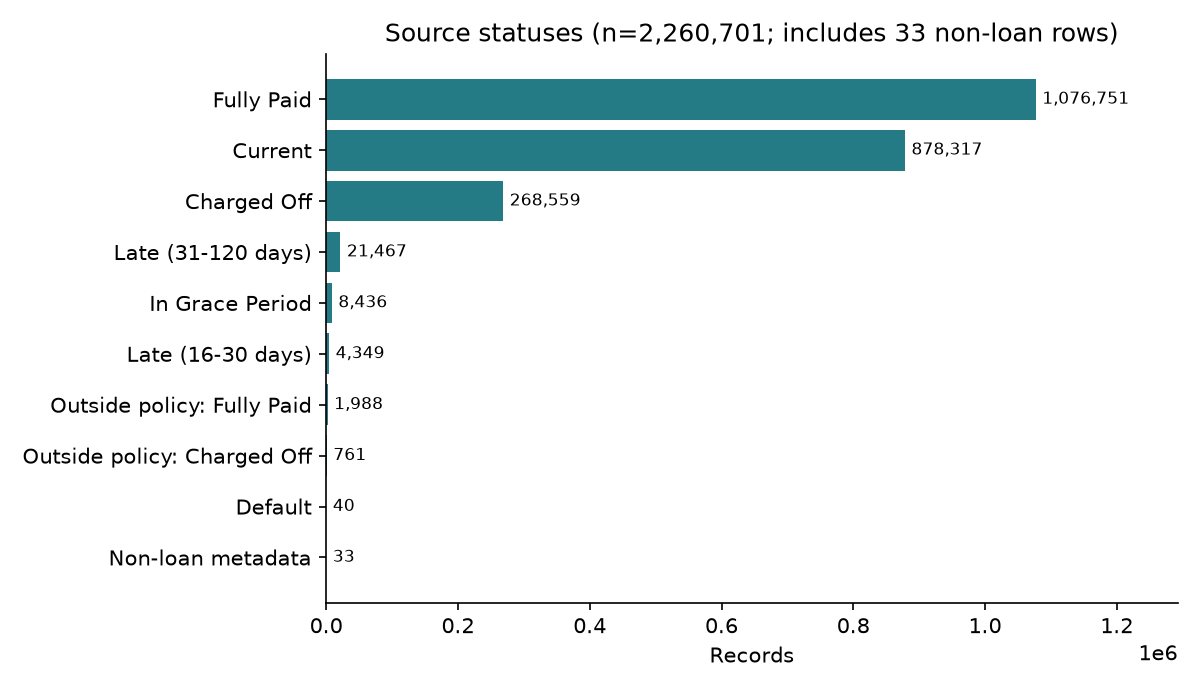
\includegraphics[width=.95\textwidth]{../figures/eda/status.png}
\caption{All source statuses. Unresolved loans make terminal-only denominator selection consequential.}\end{figure*}
\begin{figure*}[p]\centering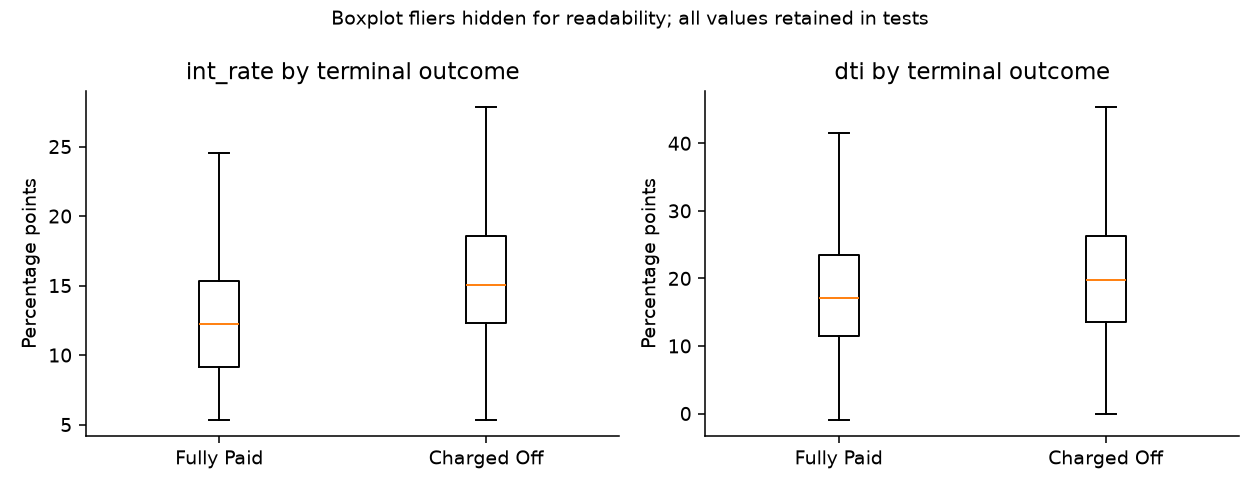
\includegraphics[width=.95\textwidth]{../figures/eda/outcome_boxplots.png}
\caption{Rate and DTI distributions by terminal outcome (1,345,310 terminal loans before variable-specific missingness). Fliers are hidden only in this plot; full observations enter tests.}\end{figure*}
\begin{figure*}[p]\centering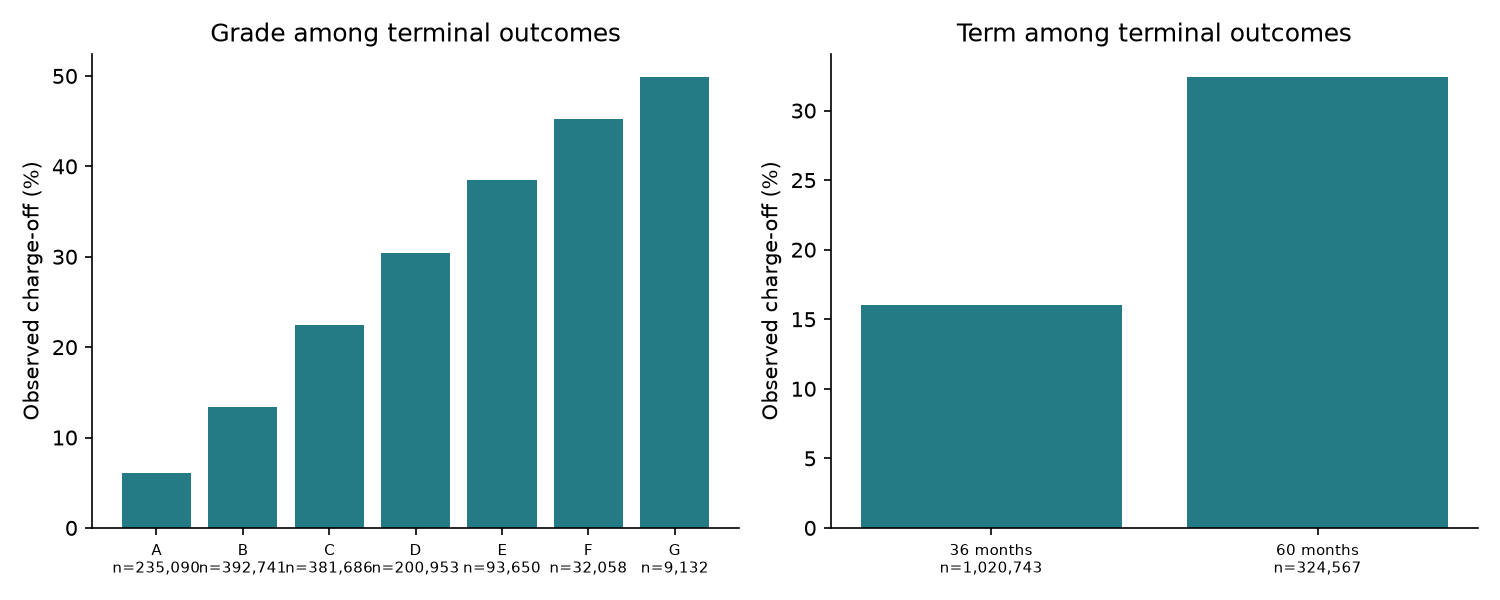
\includegraphics[width=.95\textwidth]{../figures/eda/category_rates.png}
\caption{Observed terminal charge-off proportions by grade and term. Composition and outcome maturity can confound these patterns.}\end{figure*}
<<<<<<< HEAD
\begin{figure*}[p]\centering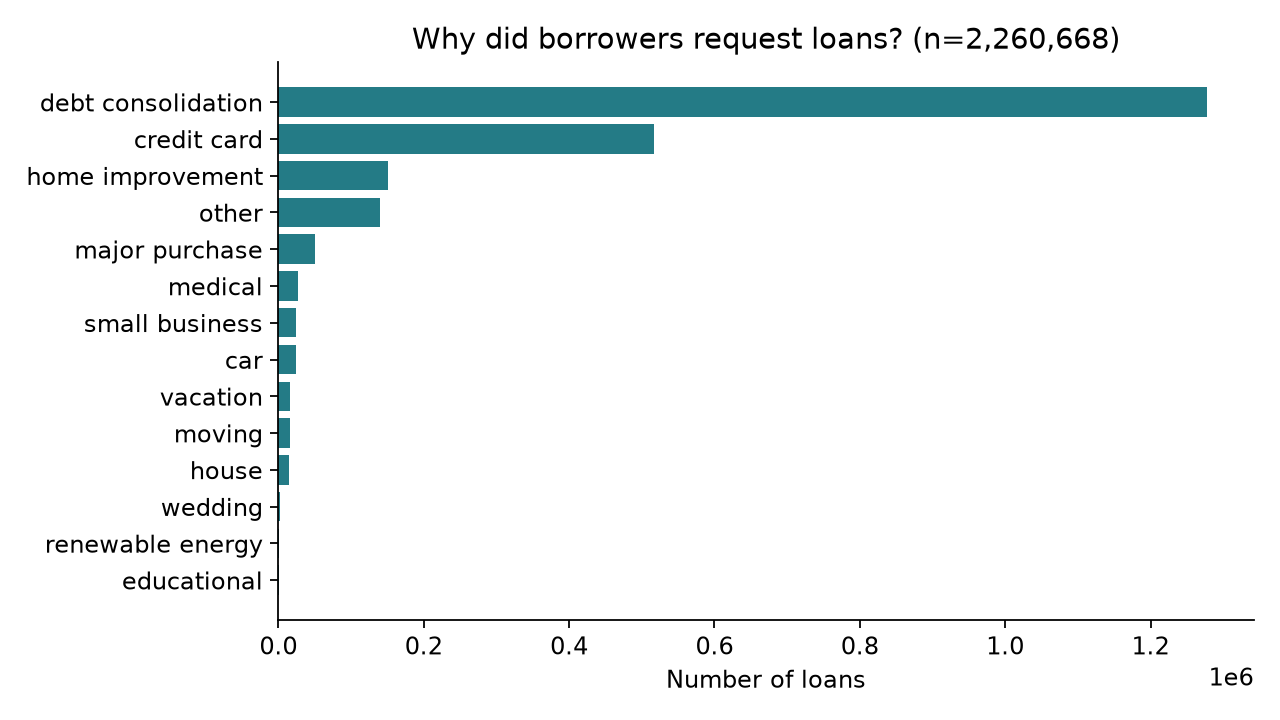
\includegraphics[width=.90\textwidth,height=.32\textheight,keepaspectratio]{../figures/eda/loan_purposes.png}
\caption{Stated borrowing purposes. The count bars show which reasons for borrowing are most common among loan records.}\end{figure*}
\begin{figure*}[p]\centering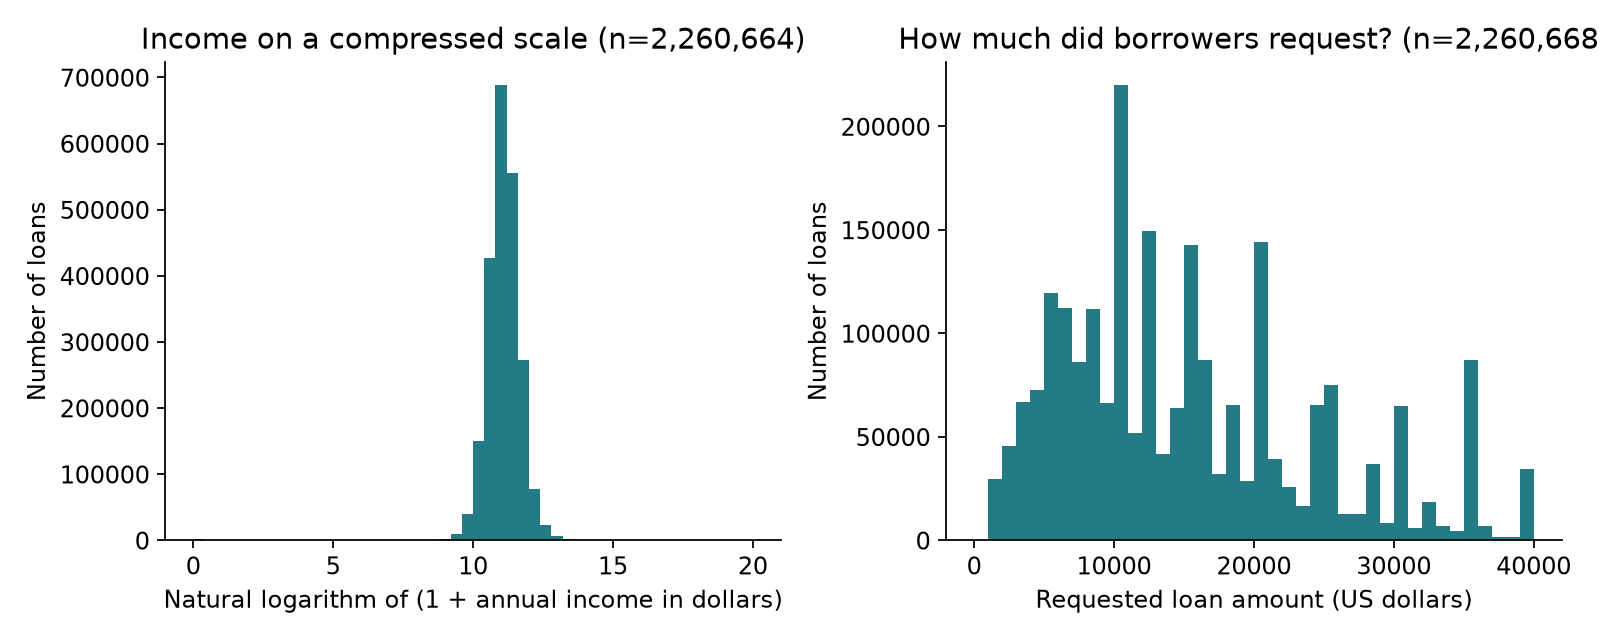
\includegraphics[width=.90\textwidth,height=.32\textheight,keepaspectratio]{../figures/eda/income_and_loan_amount.png}
\caption{Left: annual income on the natural log(1+income) scale. Right: requested loan amounts in dollars. The latter shows the size and common values of requested loans; logging income does not retain its original dollar-scale interpretation.}\end{figure*}
\begin{figure*}[p]\centering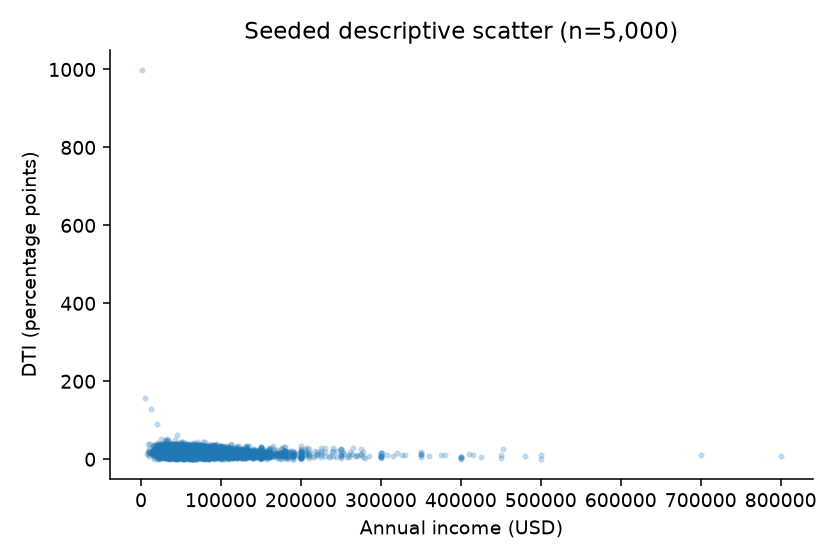
\includegraphics[width=.90\textwidth,height=.32\textheight,keepaspectratio]{../figures/eda/income_dti.png}
\caption{Seeded descriptive income--DTI scatter. Extreme values and heterogeneous borrower characteristics limit simple interpretations.}\end{figure*}
\begin{figure*}[p]\centering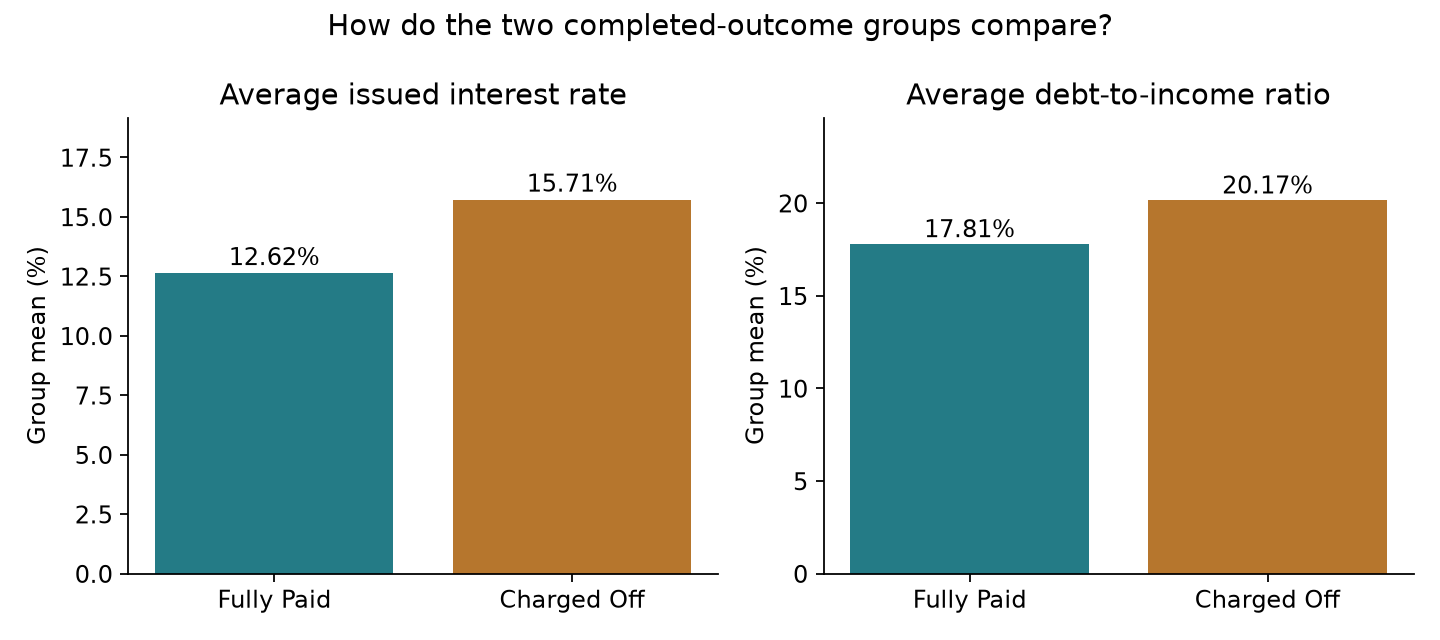
\includegraphics[width=.90\textwidth,height=.32\textheight,keepaspectratio]{../figures/eda/../inference/group_mean_comparison.png}
\caption{Average interest rate and debt-to-income ratio for Fully Paid and Charged Off loans. Both axes begin at zero. Charged Off loans have higher group averages; test tables quantify uncertainty and do not establish causation.}\end{figure*}
=======
>>>>>>> origin/main
\section{Statistical inferences}
All hypotheses were written before group tests. $\alpha=0.05$; numeric and proportion alternatives are two-sided. Chi-square uses its upper tail to detect any categorical association. Thresholds are analytical judgments, not industry standards. Loans are treated as independent for inference, an unverified assumption; large samples do not cure selection or dependence. Four tests form one Holm-adjusted family; intervals remain marginal 95\% intervals.

\subsection{Interest rate}
<<<<<<< HEAD
\begin{tabularx}{\linewidth}{@{}>{\bfseries\raggedright\arraybackslash}p{.28\linewidth} X@{}}\toprule
Notation & \(\mu_{\mathrm{CO}},\mu_{\mathrm{FP}}\): population means for CO (Charged Off) and FP (Fully Paid); \(\widehat\Delta_\mu=\bar x_{\mathrm{CO}}-\bar x_{\mathrm{FP}}\).\\\midrule
Null hypothesis \(H_0\) & \(H_0:\Delta_\mu=\mu_{\mathrm{CO}}-\mu_{\mathrm{FP}}=0\). The two population means are equal.\\\midrule
Alternative \(H_1\) & \(H_1:\Delta_\mu\ne0\). The two means differ.\\\midrule
Test / direction & Welch t; two-sided\\\midrule
Significance level & \(\alpha=0.05\); Holm adjustment across four tests.\\\midrule
Eligible sample & Charged Off: 268,559; Fully Paid: 1,076,751. Excluded terminal rows: 0.\\\midrule
Practical threshold & 1 percentage points; analyst judgement, not an industry standard.\\\midrule
Estimated difference & 3.0874 percentage points.\\\midrule
95\% CI (confidence interval) & [3.067, 3.1079] percentage points; marginal interval.\\\midrule
Test statistic & \(t=295.97\); df (degrees of freedom): 390130.\\\midrule
Probability / decision & \(p<2.23\times10^{-308}\) (floating-point underflow); reject the null hypothesis. Holm-adjusted decision also rejects.\\\midrule
Group averages & Charged Off 15.711\%; Fully Paid 12.623\%. Standard error of difference 0.010432 percentage points.\\\midrule
Why this test? & Welch t permits unequal unknown variances. A 1 percentage-point difference is the declared threshold (about 100 dollars annual simple interest per 10,000 dollars principal, not amortised cost).\\\midrule
Why not alternatives? & Known-sigma z is unsuitable; population SD (standard deviation) is unknown. Pooled t adds an unnecessary equal-variance assumption. Paired t lacks pairs. Rank tests target a different distributional question.\\\midrule
Interpretation & Charged Off loans have higher mean issued rates in this terminal sample, beyond the chosen meaningful-difference threshold.\\\bottomrule\end{tabularx}

\subsection{Debt-to-income}
\begin{tabularx}{\linewidth}{@{}>{\bfseries\raggedright\arraybackslash}p{.28\linewidth} X@{}}\toprule
Notation & \(\mu_{\mathrm{CO}},\mu_{\mathrm{FP}}\): population means for CO (Charged Off) and FP (Fully Paid); \(\widehat\Delta_\mu=\bar x_{\mathrm{CO}}-\bar x_{\mathrm{FP}}\).\\\midrule
Null hypothesis \(H_0\) & \(H_0:\Delta_\mu=\mu_{\mathrm{CO}}-\mu_{\mathrm{FP}}=0\). The two population means are equal.\\\midrule
Alternative \(H_1\) & \(H_1:\Delta_\mu\ne0\). The two means differ.\\\midrule
Test / direction & Welch t; two-sided\\\midrule
Significance level & \(\alpha=0.05\); Holm adjustment across four tests.\\\midrule
Eligible sample & Charged Off: 268,488; Fully Paid: 1,076,448. Excluded terminal rows: 374.\\\midrule
Practical threshold & 2 percentage points; analyst judgement, not an industry standard.\\\midrule
Estimated difference & 2.3596 percentage points.\\\midrule
95\% CI (confidence interval) & [2.3103, 2.4089] percentage points; marginal interval.\\\midrule
Test statistic & \(t=93.8212\); df (degrees of freedom): 390672.\\\midrule
Probability / decision & \(p<2.23\times10^{-308}\) (floating-point underflow); reject the null hypothesis. Holm-adjusted decision also rejects.\\\midrule
Group averages & Charged Off 20.171\%; Fully Paid 17.812\%. Standard error of difference 0.02515 percentage points.\\\midrule
Why this test? & Welch t on the original scale. Threshold: 2 percentage points (100 dollars monthly debt per 5,000 dollars monthly income illustrates scale). Extreme values and missingness warrant sensitivity analysis.\\\midrule
Why not alternatives? & Pooled, known-sigma and paired tests have the same limitations as for rate. Log/rank analyses change the estimand; primary inference retains original values.\\\midrule
Interpretation & Charged Off loans have higher mean DTI in this terminal sample, beyond the chosen meaningful-difference threshold.\\\bottomrule\end{tabularx}

\subsection{Grade}
\begin{tabularx}{\linewidth}{@{}>{\bfseries\raggedright\arraybackslash}p{.28\linewidth} X@{}}\toprule
Notation & \(G\): recorded grade; \(Y\): terminal outcome; \(\perp\) means statistical independence. \(V=\sqrt{\chi^2/N}\) is Cramer\textquotesingle s association measure for this two-outcome table.\\\midrule
Null hypothesis \(H_0\) & \(H_0:G\perp Y\). Grade and terminal outcome are independent.\\\midrule
Alternative \(H_1\) & \(H_1:G\not\perp Y\). Grade and terminal outcome are associated.\\\midrule
Test / direction & Chi-square independence; upper-tail independence test\\\midrule
Significance level & \(\alpha=0.05\); Holm adjustment across four tests.\\\midrule
Eligible sample & 1,345,310 loans, seven grades, two outcomes. Excluded terminal rows: 0.\\\midrule
Practical threshold & 0.1 Cramer's V (association magnitude); analyst judgement, not an industry standard.\\\midrule
Association size & 0.26191 Cramer's V (association magnitude).\\\midrule
95\% CI (confidence interval) & [0.26029, 0.26345] Cramer's V (association magnitude); marginal interval.\\\midrule
Test statistic & \(\chi^2=92284.3\); df (degrees of freedom): 6.\\\midrule
Probability / decision & \(p<2.23\times10^{-308}\) (floating-point underflow); reject the null hypothesis. Holm-adjusted decision also rejects.\\\midrule
Approximation check & Smallest expected count 1823; above five.\\\midrule
Why this test? & Pearson chi-square on the grade-by-outcome counts; Cramer's V measures magnitude. V=0.10 is a weak exploratory convention, not a validated business threshold. A 1,000-draw IID (independent and identically distributed) multinomial bootstrap gives its interval (extension).\\\midrule
Why not alternatives? & A correlation test would impose an arbitrary numeric grade spacing. Sparse-table exact methods are alternatives when expected counts fail; all expected cells are checked. No post-hoc grade tests are counted.\\\midrule
Interpretation & Grade and terminal outcome are associated; V exceeds the exploratory magnitude threshold. This is not independent causal evidence beyond the rate comparison.\\\bottomrule\end{tabularx}

\subsection{Term}
\begin{tabularx}{\linewidth}{@{}>{\bfseries\raggedright\arraybackslash}p{.28\linewidth} X@{}}\toprule
Notation & \(p_{60},p_{36}\): population charge-off proportions among terminal loans of each term; \(\widehat\Delta_p=\widehat p_{60}-\widehat p_{36}\).\\\midrule
Null hypothesis \(H_0\) & \(H_0:\Delta_p=p_{60}-p_{36}=0\). The two population charge-off proportions are equal.\\\midrule
Alternative \(H_1\) & \(H_1:\Delta_p\ne0\). The two charge-off proportions differ.\\\midrule
Test / direction & Two-proportion z; two-sided\\\midrule
Significance level & \(\alpha=0.05\); Holm adjustment across four tests.\\\midrule
Eligible sample & 60 months: 324,567; 36 months: 1,020,743. Excluded terminal rows: 0.\\\midrule
Practical threshold & 2 percentage points; analyst judgement, not an industry standard.\\\midrule
Estimated difference & 16.452 percentage points.\\\midrule
95\% CI (confidence interval) & [16.276, 16.628] percentage points; marginal interval.\\\midrule
Test statistic & \(z=204.25\); df (degrees of freedom): not applicable.\\\midrule
Probability / decision & \(p<2.23\times10^{-308}\) (floating-point underflow); reject the null hypothesis. Holm-adjusted decision also rejects.\\\midrule
Group event rates & 60 months 32.445\%; 36 months 15.993\%.\\\midrule
Approximation check & Smallest expected count 64792; above five.\\\midrule
Why this test? & Pooled-null two-proportion z; unpooled large-sample difference interval. Event = Charged Off, denominator = terminal loans of each term. Threshold .02 means 2 additional events per 100 terminal loans.\\\midrule
Why not alternatives? & The uncorrected 2x2 chi-square is equivalent (z squared), checked but not counted as another finding. Fisher exact is unnecessary when expected cells are adequate. A t test is not the natural binary-count method.\\\midrule
Interpretation & The 60-month terminal group has a higher observed charge-off proportion by about 16.45 percentage points. Selection and maturity prevent a causal interpretation.\\\bottomrule\end{tabularx}
=======
\textbf{a) Hypotheses and choice.} \(H_0:\mu_{CO}-\mu_{FP}=0;\quad H_1:\mu_{CO}-\mu_{FP}\ne0\)

Welch t permits unequal unknown variances. A 1 percentage-point difference is the declared threshold (about 100 dollars annual simple interest per 10,000 dollars principal, not amortised cost).

\textbf{b) Alternatives.} Known-sigma z is unsuitable; population SD is unknown. Pooled t adds an unnecessary equal-variance assumption. Paired t lacks pairs. Rank tests target a different distributional question.

\textbf{c) Result.} n(CO)=268,559, n(FP)=1,076,751; excluded terminal rows=0. Estimate 3.0874; 95\% CI [3.067, 3.1079]; statistic 295.97; df 390,130; p < 2.23e-308 (floating-point underflow). Reject H0. Holm p < 2.23e-308 (floating-point underflow). CI beyond positive threshold.

Group means 15.711, 12.623; SDs 4.9104, 4.5272; SE 0.010432.

Charged Off loans have higher mean issued rates in this terminal sample, beyond the chosen meaningful-difference threshold.


\subsection{Debt-to-income}
\textbf{a) Hypotheses and choice.} \(H_0:\mu_{CO}-\mu_{FP}=0;\quad H_1:\mu_{CO}-\mu_{FP}\ne0\)

Welch t on the original scale. Threshold: 2 percentage points (100 dollars monthly debt per 5,000 dollars monthly income illustrates scale). Extreme values and missingness warrant sensitivity analysis.

\textbf{b) Alternatives.} Pooled, known-sigma and paired tests have the same limitations as for rate. Log/rank analyses change the estimand; primary inference retains original values.

\textbf{c) Result.} n(CO)=268,488, n(FP)=1,076,448; excluded terminal rows=374. Estimate 2.3596; 95\% CI [2.3103, 2.4089]; statistic 93.8212; df 390,672; p < 2.23e-308 (floating-point underflow). Reject H0. Holm p < 2.23e-308 (floating-point underflow). CI beyond positive threshold.

Group means 20.171, 17.812; SDs 11.832, 10.936; SE 0.02515.

Charged Off loans have higher mean DTI in this terminal sample, beyond the chosen meaningful-difference threshold.


\subsection{Grade}
\textbf{a) Hypotheses and choice.} \(H_0:\text{independence};\quad H_1:\text{association}\)

Pearson chi-square on the grade-by-outcome counts; Cramer's V measures magnitude. V=0.10 is a weak exploratory convention, not a validated business threshold. A 1,000-draw IID multinomial bootstrap gives its interval (extension).

\textbf{b) Alternatives.} A correlation test would impose an arbitrary numeric grade spacing. Sparse-table exact methods are alternatives when expected counts fail; all expected cells are checked. No post-hoc grade tests are counted.

\textbf{c) Result.} N=1,345,310; excluded terminal rows=0. Estimate 0.26191; 95\% CI [0.26029, 0.26345]; statistic 92284.3; df 6; p < 2.23e-308 (floating-point underflow). Reject H0. Holm p < 2.23e-308 (floating-point underflow). CI beyond positive threshold.

Minimum expected cell count: 1823.

Grade and terminal outcome are associated; V exceeds the exploratory magnitude threshold. This is not independent causal evidence beyond the rate comparison.


\subsection{Term}
\textbf{a) Hypotheses and choice.} \(H_0:p_{60}-p_{36}=0;\quad H_1:p_{60}-p_{36}\ne0\)

Pooled-null two-proportion z; unpooled large-sample difference interval. Event = Charged Off, denominator = terminal loans of each term. Threshold .02 means 2 additional events per 100 terminal loans.

\textbf{b) Alternatives.} The uncorrected 2x2 chi-square is equivalent (z squared), checked but not counted as another finding. Fisher exact is unnecessary when expected cells are adequate. A t test is not the natural binary-count method.

\textbf{c) Result.} n(60)=324,567, n(36)=1,020,743; excluded terminal rows=0. Estimate 0.16452; 95\% CI [0.16276, 0.16628]; statistic 204.25; df not applicable; p < 2.23e-308 (floating-point underflow). Reject H0. Holm p < 2.23e-308 (floating-point underflow). CI beyond positive threshold.

Minimum expected cell count: 64792.

Observed event proportions: 0.32445 (60 months), 0.15993 (36 months). Difference/interval above are proportions, not percentage points.

The 60-month terminal group has a higher observed charge-off proportion by about 16.45 percentage points. Selection and maturity prevent a causal interpretation.
>>>>>>> origin/main

\textbf{Calculation audit.} Welch: $SE=\sqrt{s_A^2/n_A+s_B^2/n_B}$, $t=\hat\Delta/SE$, with Satterthwaite df and t-quantile interval. Proportion z uses pooled $p$ under the null; its interval uses the separate estimated proportions. Chi-square sums $(O-E)^2/E$, with $E=$ row total times column total divided by $N$, and df=$(r-1)(c-1)$. Full intermediate values, formulas and alternatives are in methodology\_and\_results.md and the source functions.

\textbf{Sensitivity.}
 int\_rate: capping at 26.3 gives difference 3.037, CI [3.0172, 3.0568].
 dti: capping at 38.47 gives difference 2.2908, CI [2.2545, 2.327].

The cap changes the estimand; it is not a correction of proven errors. Issue-year/term rates are provided to inspect composition, not to claim censoring is resolved.
\section{Limitations}
Accepted loans exclude rejected applications. Terminal selection excludes unfinished loans and can overrepresent early charge-offs, particularly for newer long-term loans. These are conditional associations, not lifetime default rates or causal effects. Grade and rate reflect related underwriting information; shared borrowers and macroeconomic shocks can violate independence. No reliable borrower identifier was established. Complete cases can be selective, and extreme DTI values require historical documentation.

<<<<<<< HEAD
Holm addresses multiplicity conditional on valid p-values; it does not remove confounding. Subjective practical thresholds should be challenged. Historical file provenance, extraction date and licence are incomplete. The supplied lecture PDFs (Portable Document Format files), quizzes and practice problems were absent, so exact lecture mapping and the 80\% syllabus target cannot be verified. Bootstrap and Holm are labelled extensions. No classifier is claimed.

\textbf{References and code.} Supplied CSE558 guidelines/template; supplied preliminary LendingClub profile; the local CSV identified by its saved hash. Historical grade context: LendingClub SEC prospectus (2011), \url{https://www.sec.gov/Archives/edgar/data/1409970/000095012311058394/c18687e424b3.htm}. This source does not verify definitions for every vintage. See references.md, README.md and src/statistical\_tests.py. Project code and README: \url{https://github.com/krishiv-rtx/Data-Science-Project}.
\clearpage\onecolumn\section{Plain-language reference}\small
\textbf{Selected source and derived attributes.} The complete source inventory is in attributes\_plain\_language.md. Historical definitions remain subject to the provenance caveat.
\begin{tabularx}{\linewidth}{@{}l X X@{}}\toprule Attribute & Plain meaning & What it tells us\\\midrule
id & Loan identifier & Tracks a loan; has no numerical risk interpretation.\\
loan\_status & Recorded loan outcome & Defines Fully Paid and Charged Off groups; Current is unresolved.\\
issue\_d & Loan issue month & Shows loan vintage and helps explain maturity differences.\\
loan\_amnt & Requested loan amount, in dollars & Shows the size of the loan, not the amount repaid.\\
int\_rate & Issued annual interest rate, in percent & The price charged for borrowing; tested between outcome groups.\\
dti & Debt-to-income ratio, in percent & A debt-burden measure; higher means more debt relative to income.\\
annual\_inc & Reported annual income, dollars per year & Borrower income scale; zero/extreme values need context.\\
fico\_range\_low & Lower end of the origination credit-score band & An approximate credit-score range endpoint, not the exact score.\\
revol\_util & Revolving credit utilisation, in percent & How much of available revolving credit is used; unusually large values need review.\\
grade & Recorded loan grade, A through G & An ordered underwriting label, not an equally spaced number.\\
term & Scheduled loan duration, in months & The comparison uses 36-month and 60-month loans.\\
home\_ownership & Reported housing situation & For example, rent, mortgage or own; a category, not wealth itself.\\
verification\_status & Recorded income-verification category & Describes verification status; does not guarantee truthful income.\\
purpose & Stated reason for borrowing & For example, debt consolidation; self-reported category.\\
application\_type & Individual or joint application & Helps interpret why joint-applicant fields may be missing.\\
charged\_off & Derived 1 for Charged Off, 0 for Fully Paid & Defined only in the selected terminal-outcome sample.\\\bottomrule\end{tabularx}
\medskip
\textbf{Acronym directory and statistical shorthand.}\par\begin{tabularx}{\linewidth}{@{}l X@{}}\toprule Short form & Expanded meaning\\\midrule
DTI & Debt-to-income ratio\\
FICO & Fair Isaac Corporation credit score\\
CI & Confidence interval\\
SD & Standard deviation\\
SE & Standard error\\
df & Degrees of freedom\\
IQR & Interquartile range\\
CO & Charged Off\\
FP & Fully Paid\\
EDA & Exploratory data analysis\\
H0 & Null hypothesis\\
H1 & Alternative hypothesis\\
IID & Independent and identically distributed\\
USD & United States dollars\\
CSV & Comma-separated values\\
SHA-256 & Secure Hash Algorithm, 256-bit\\\bottomrule\end{tabularx}

\medskip\textbf{Mathematical notation.} \(\mu\): population mean; \(\bar x\): sample mean; \(p\): population proportion (or a p-value when explicitly labelled); \(\widehat p\): sample proportion; \(\Delta\): difference; \(s\): SD (standard deviation); \(\mathrm{SE}\): standard error; \(\nu\): degrees of freedom; \(n,N\): sample counts; \(\alpha\): significance level; \(t,z,\chi^2\): test statistics. \(H_0\) is the null hypothesis; \(H_1\) is the alternative hypothesis. Welch, Holm and Cramer are names, not acronyms.
=======
Holm addresses multiplicity conditional on valid p-values; it does not remove confounding. Subjective practical thresholds should be challenged. Historical file provenance, extraction date and licence are incomplete. The supplied lecture PDFs, quizzes and practice problems were absent, so exact lecture mapping and the 80\% syllabus target cannot be verified. Bootstrap and Holm are labelled extensions. No classifier is claimed.

\textbf{References and code.} Supplied CSE558 guidelines/template; supplied preliminary LendingClub profile; the local CSV identified by its saved hash. Historical grade context: LendingClub SEC prospectus (2011), \url{https://www.sec.gov/Archives/edgar/data/1409970/000095012311058394/c18687e424b3.htm}. This source does not verify definitions for every vintage. See references.md, README.md and src/statistical\_tests.py. Replace the code URL and team metadata fields before submission.
>>>>>>> origin/main
\end{document}
